\chapter{Patrones GoF}
\section{Patrones Creacionales}
Los patrones de diseño creacional resumen el proceso de creación de instancias. Ayudan a que un sistema sea independiente de cómo se crean, componen y representan sus objetos. Un patrón de creación de clases utiliza la herencia para variar la clase que está instanciada, mientras que un patrón de creación de objetos delegará la creación de instancias en otro objeto. Los patrones de creación se vuelven importantes a medida que los sistemas evolucionan para depender más de la composición de objetos que de la herencia de clase. Tal como sucede, el énfasis se aparta de la codificación rígida de un conjunto fijo de comportamientos para definir un conjunto más pequeño de comportamientos fundamentales que se pueden componer en cualquier cantidad de comportamientos más complejos. Por lo tanto, crear objetos con comportamientos particulares requiere algo más que simplemente crear una instancia de una clase. Hay dos temas recurrentes en estos patrones. Primero, todos encapsulan el conocimiento sobre las clases concretas que usa el sistema. En segundo lugar, ocultan cómo se crean y se crean las instancias de estas clases. Todo el sistema en general sabe acerca de los objetos es sus interfaces según lo definido por las clases abstractas. En consecuencia, los patrones creacionales le dan mucha flexibilidad en lo que se crea, quién lo crea, cómo se crea y cuándo. Le permiten configurar un sistema con objetos "producto" que varían ampliamente en estructura y funcionalidad. La configuración puede ser estática (es decir, especificada en tiempo de compilación) o dinámica (en tiempo de ejecución).\cite{gof}
\subsection{Patrón Prototype}
\subsubsection{Descripción}
Este patrón tiene or objetivo crear objetos prediseñados sin conocer detalles de cómo crearlos, en diversos casos el costo de crear un objeto elevado, especialmente cuando se deben especificar un gran conjunto de productos. Para este contexto, resulta conveniente, clonar dicho objeto, aprovecharse de la estructura original y ajustarle un nuevo propósito. 

\paragraph{Estructura}

\begin{figure}[th!]
	\centering
	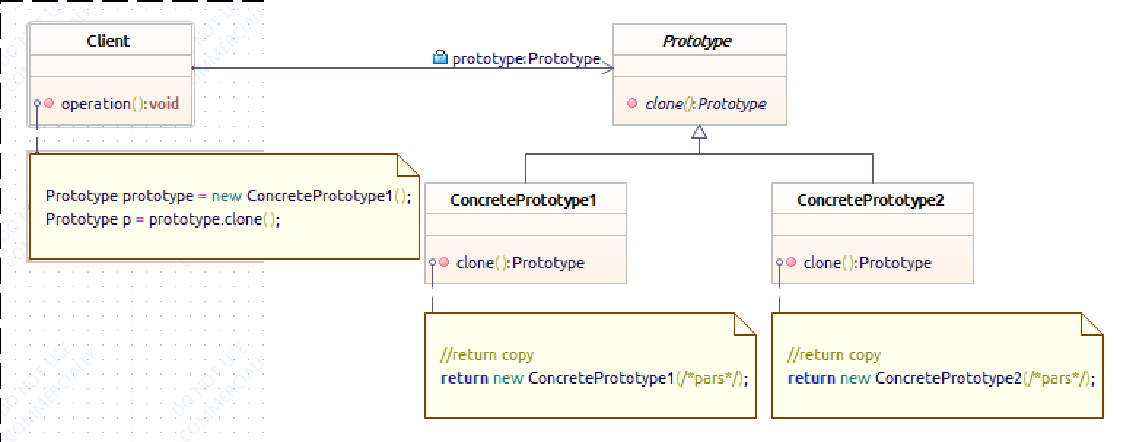
\includegraphics[width=.7\linewidth]{imagenes/Patrones/Prototype.pdf}
	\caption{Estructura del patrón Prototype.\cite{gof}}	
\end{figure}

\paragraph{Actores}

\begin{itemize}
	\item \textbf{Prototype}:Declara la interface del objeto que se clona.
	\item \textbf{Concrete Prototype}: Implementa las operaciones para la clonación del objeto prototipo.
	\item \textbf{Cliente}: Accede a la generación de los objetos clonados.
\end{itemize}


\subsubsection{Caso de Uso}

\begin{figure}[th!]
	\centering
	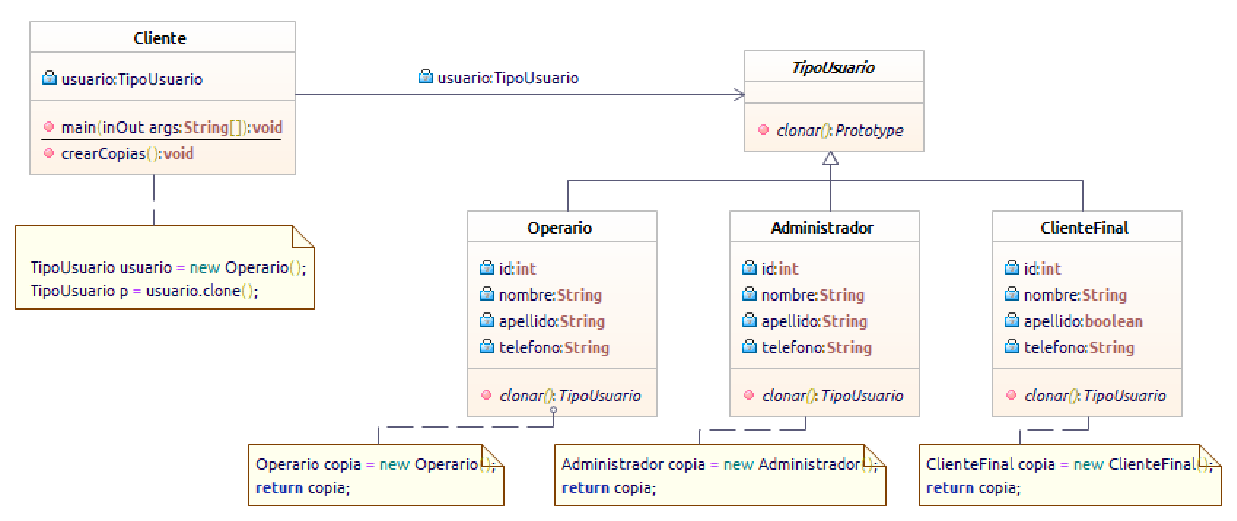
\includegraphics[width=.7\linewidth]{imagenes/Patrones/Prototype_caso.pdf}
	\caption{Estructura del patrón Prototype caso de uso.\cite{gof}}	
\end{figure}



\subsection{Patrón Fabrica Abstracta}
\subsubsection{Descripción}
Este patrón al igual que todos los de tipo creacional, tiene por objetivo, solucionar le problema de código duro, el cúal es un escenario típico donde se crean instrucciones y objetos que al cerrarlos, no pueden cambiarse.
En dicho patrón, el cliente no quiere caer en código duro para la creación de productos concretos, por lo que lo hace a través de un conjunto de Fábrica Abstractas, que viene a ser la la envoltura, lo que facilita en gran medida, que cuando las familias de productos evoluciones, las familias se crean a través de fabricas abstractas.

\paragraph{Estructura}

\begin{figure}[th!]
	\centering
	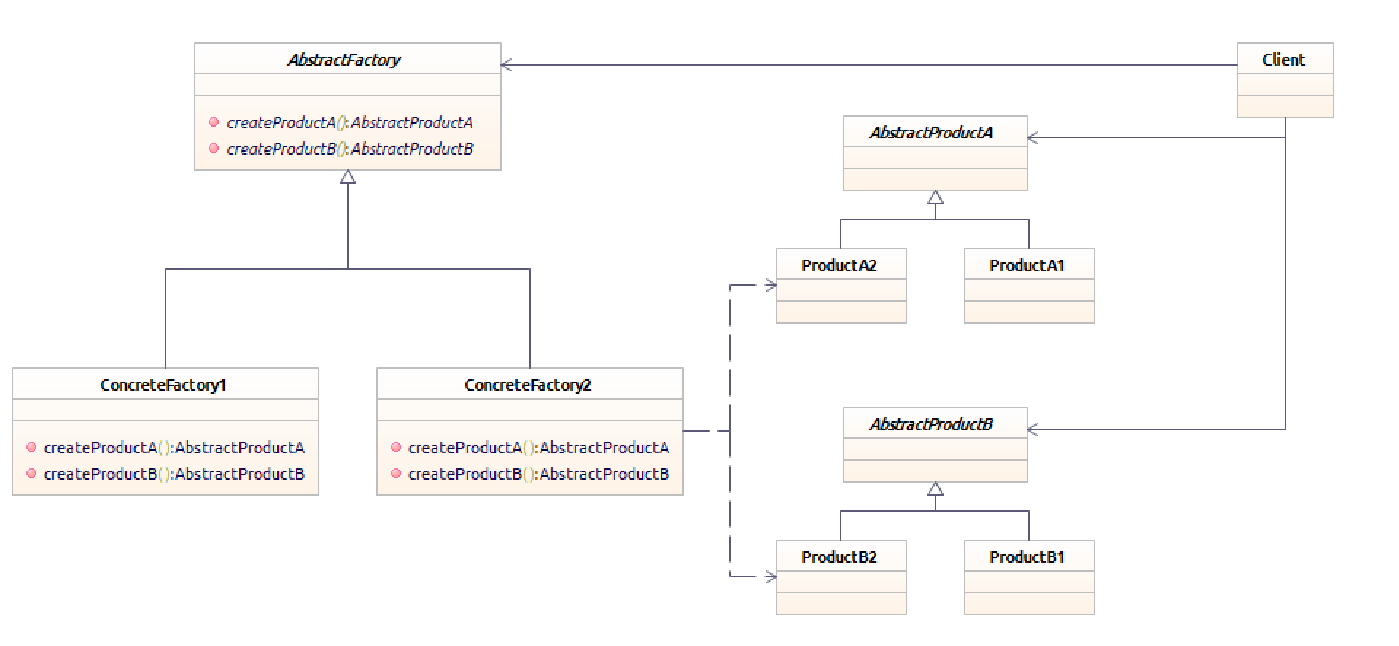
\includegraphics[width=.7\linewidth]{imagenes/Patrones/Fabrica.pdf}
	\caption{Estructura del patrón Fabrica Abstracta.\cite{gof}}	
\end{figure}

\paragraph{Actores}

\begin{itemize}
	\item \textbf{Fabrica Abstracta}: Declara una interfaz para operaciones que crean objetos de productos abstractos.
	\item \textbf{Fabrica Concreta}: Implementa las operaciones para crear objetos productos concretos.
	\item \textbf{Producto Abstracto}: Declara la interfaz para un tipo de objeto producto.
	\item \textbf{Producto Concreto}: Define un objeto producto para que sea creado por la fabrica conrrespondiente. Implementa la interfaz Producto abstracto.
	\item \textbf{Cliente}: Solo usa la interfaces declaradas por las clases Fabrica Abstracta y Producto Abstracto.
	
\end{itemize}


\subsubsection{Caso de Uso}
\begin{figure}[th!]
	\centering
	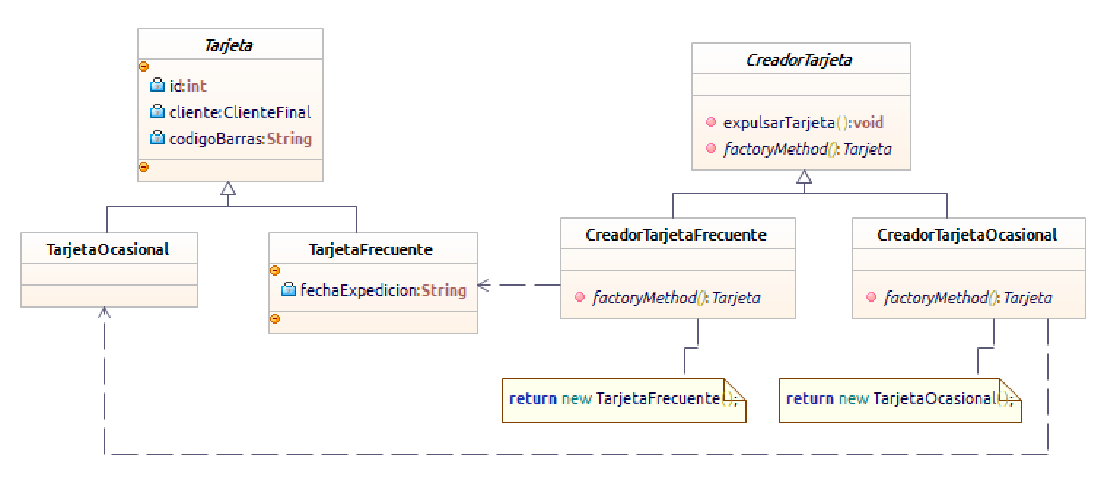
\includegraphics[width=.7\linewidth]{imagenes/Patrones/Fabrica_caso.pdf}
	\caption{Estructura del patrón Fabrica Abstracta caso de uso.\cite{gof}}	
\end{figure}

\section{Patrones de Comportamiento}
Los patrones de comportamiento se relacionan con los algoritmos y la asignación de responsabilidades entre los objetos. Los patrones de comportamiento describen no solo patrones de objetos o clases sino también los patrones de comunicación entre ellos. Estos patrones caracterizan el flujo de control complejo que es difícil de seguir en el tiempo de ejecución. Desvían su enfoque del flujo de control para permitirle concentrarse en el modo en que los objetos están interconectados. Los patrones de objetos de comportamiento utilizan la composición de objetos en lugar de la herencia. Algunos describen cómo un grupo de objetos similares cooperan para realizar una tarea que ningún objeto individual puede llevar a cabo por sí mismo. Un tema importante aquí es cómo los objetos de pares se conocen unos a otros. Los pares podrían mantener referencias explícitas entre sí, pero eso aumentaría su acoplamiento. En el extremo, cada objeto sabría sobre cada otro.\cite{gof}
\subsection{Patrón Strategy}

\subsubsection{Descripción}

\paragraph{Estructura}

\begin{figure}[th!]
	\centering
	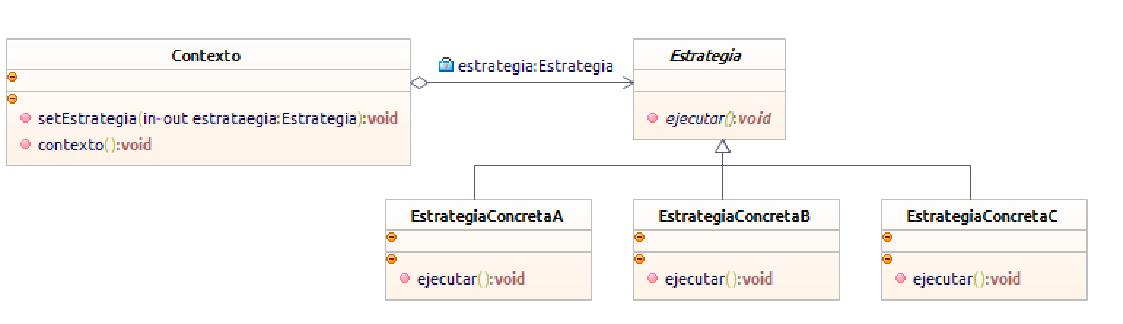
\includegraphics[width=.7\linewidth]{imagenes/Patrones/Strategy.pdf}
	\caption{Estructura del patrón Strategy.\cite{gof}}	
\end{figure}

\paragraph{Actores}

\begin{itemize}
	\item \textbf{Proxy}: Controla el acceso al sujeto real y puede ser responsable de crearlo y eliminarlo.
	\item \textbf{Sujeto}:Define la interfaz común para las clase SujetoReal y Proxy para que un Proxy se pueda usar en cualquier lugar donde se espere un SujetoReal.
	\item \textbf{Sujeto Real}:Define el objeto real al cual representa el Proxy.
\end{itemize}


\subsubsection{Caso de Uso}
\begin{figure}[th!]
	\centering
	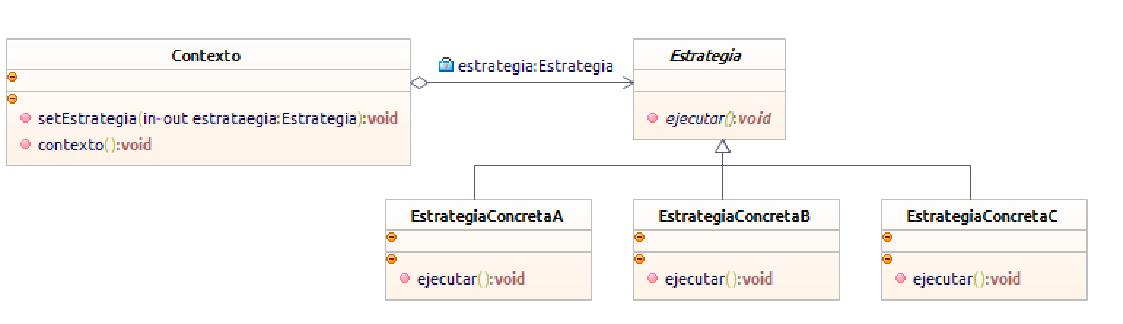
\includegraphics[width=.7\linewidth]{imagenes/Patrones/Strategy_caso.pdf}
	\caption{Estructura del patrón Strategy caso de uso.\cite{gof}}	
\end{figure}

\subsection{Patrón State}

\subsubsection{Descripción}

\paragraph{Estructura}

\begin{figure}[th!]
	\centering
	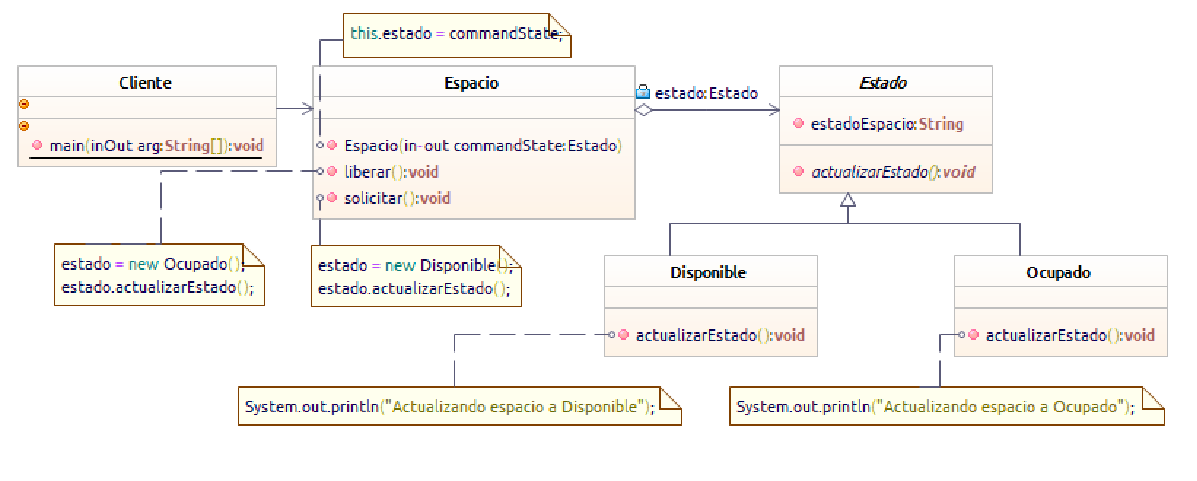
\includegraphics[width=.7\linewidth]{imagenes/Patrones/State.pdf}
	\caption{Estructura del patrón State.\cite{gof}}	
\end{figure}

\paragraph{Actores}

\begin{itemize}
	\item \textbf{Proxy}: Controla el acceso al sujeto real y puede ser responsable de crearlo y eliminarlo.
	\item \textbf{Sujeto}:Define la interfaz común para las clase SujetoReal y Proxy para que un Proxy se pueda usar en cualquier lugar donde se espere un SujetoReal.
	\item \textbf{Sujeto Real}:Define el objeto real al cual representa el Proxy.
\end{itemize}


\subsubsection{Caso de Uso}
\begin{figure}[th!]
	\centering
	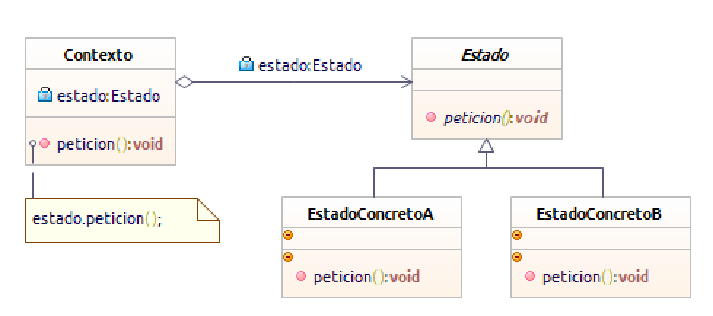
\includegraphics[width=.7\linewidth]{imagenes/Patrones/State_caso.pdf}
	\caption{Estructura del patrón State caso de uso.\cite{gof}}	
\end{figure}
\subsection{Patrón Cadena de Responsabilidad}

\subsubsection{Descripción}

\paragraph{Estructura}

\begin{figure}[th!]
	\centering
	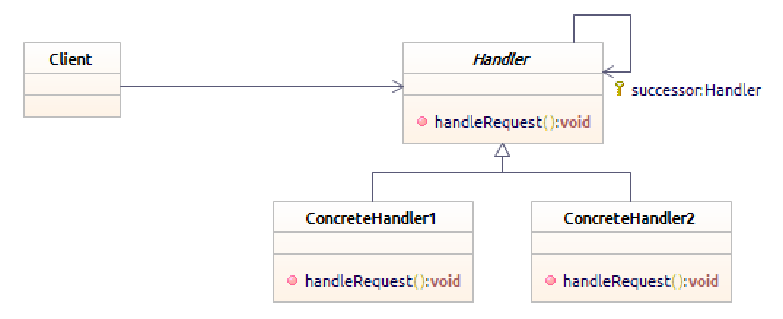
\includegraphics[width=.7\linewidth]{imagenes/Patrones/Cadena.pdf}
	\caption{Estructura del patrón Cadena de Responsabilidad.\cite{gof}}	
\end{figure}

\paragraph{Actores}

\begin{itemize}
	\item \textbf{Proxy}: Controla el acceso al sujeto real y puede ser responsable de crearlo y eliminarlo.
	\item \textbf{Sujeto}:Define la interfaz común para las clase SujetoReal y Proxy para que un Proxy se pueda usar en cualquier lugar donde se espere un SujetoReal.
	\item \textbf{Sujeto Real}:Define el objeto real al cual representa el Proxy.
\end{itemize}


\subsubsection{Caso de Uso}
\begin{figure}[th!]
	\centering
	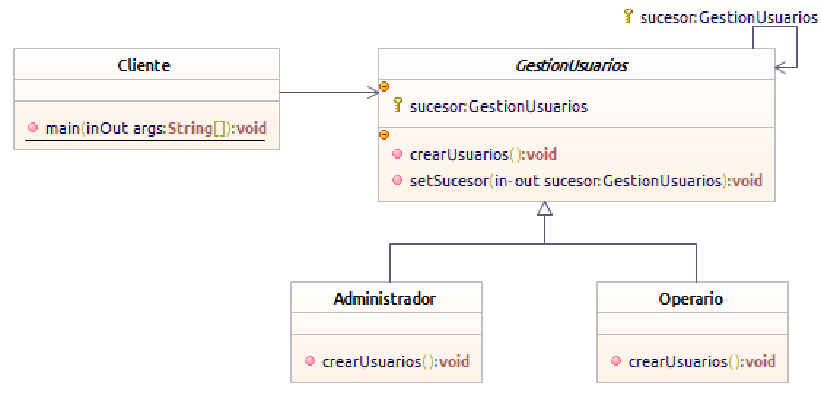
\includegraphics[width=.7\linewidth]{imagenes/Patrones/Cadena_caso.pdf}
	\caption{Estructura del patrón Cadena de Responsabilidad caso de uso.\cite{gof}}	
\end{figure}

\section{Patrones Estructurales}
Los patrones estructurales se refieren a cómo se componen las clases y los objetos para formar estructuras más grandes. Los patrones de clases estructurales utilizan la herencia para componer interfaces o implementaciones. Como ejemplo simple, considere cómo la herencia múltiple mezcla dos o más clases en una sola. El resultado es una clase que combina las propiedades de sus clases principales. Este patrón es particularmente útil para hacer que las bibliotecas de clases desarrolladas independientemente trabajen juntas. En lugar de componer interfaces o implementaciones, los patrones de objetos estructurales describen formas de componer objetos para realizar nuevas funcionalidades. La flexibilidad añadida de la composición de objetos proviene de la capacidad de cambiar la composición en tiempo de ejecución, lo que es imposible con la composición de clase estática.\cite{gof}
\subsection{Patrón Bridge}


\subsubsection{Descripción}
Cuando una abstracción puede tener una de varias implementaciones posibles, la forma habitual de acomodarlas es utilizar la herencia. Una clase abstracta define la interfaz a la abstracción, y las subclases concretas la implementan de diferentes maneras. Pero este enfoque no siempre es lo suficientemente flexible. La herencia vincula una implementación a la abstracción de forma permanente, lo que dificulta la modificación, ampliación y reutilización de abstracciones e implementaciones de forma independiente.

\paragraph{Estructura}

\begin{figure}[th!]
	\centering
	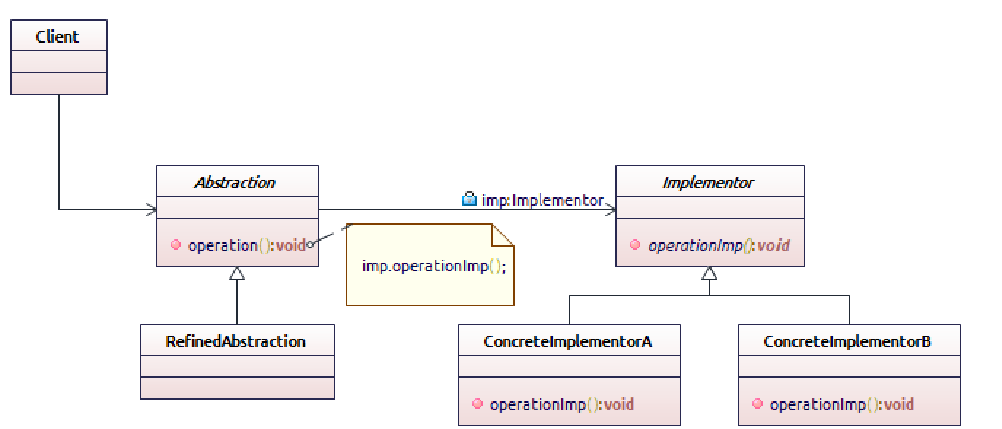
\includegraphics[width=.7\linewidth]{imagenes/Patrones/Bridge.pdf}
	\caption{Estructura del patrón Bridge.\cite{gof}}	
\end{figure}

\paragraph{Actores}

\begin{itemize}
	\item \textbf{Abstracción}: Define la interfaz de abstracción y mantiene una referencia a un objeto de tipo Implementador.
	\item \textbf{Abstracción refinada}: Amplía la interfaz definida por la Abstracción.
	\item \textbf{Implementador}: Define la interfaz para las clases de implementación. Esta interfaz no tiene que corresponderse exactamente con la interfaz de Abstracción, de hecho, las dos interfaces pueden ser bastante diferentes. Normalmente, la interfaz del implementador proporciona solo operaciones primitivas, y la abstracción define operaciones de nivel superior basadas en estas primitivas.
	\item \textbf{implementador concreto}: El implementador concreto implementa la interfaz del implementador y define su implementación concreta.
\end{itemize}


\subsubsection{Caso de Uso}
\begin{figure}[th!]
	\centering
	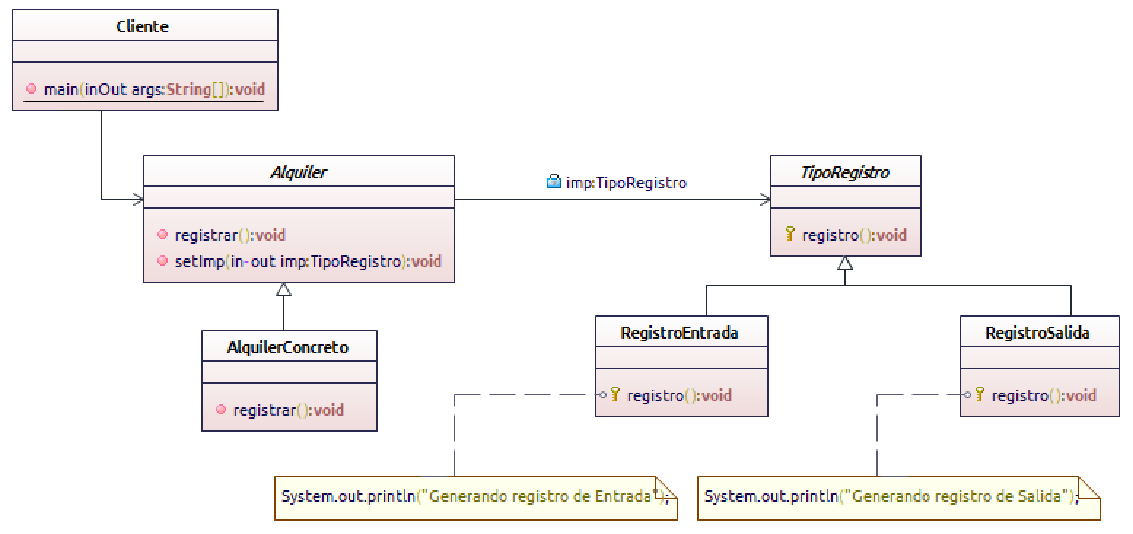
\includegraphics[width=.7\linewidth]{imagenes/Patrones/Bridge_caso.pdf}
	\caption{Estructura del patrón Bridge caso de uso.\cite{gof}}	
\end{figure}
\subsection{Patrón Proxy}

\subsubsection{Descripción}
El patron Proxy es un patrón que permite controlar el acceso a un objeto, esto  mediante una entidad intermediara, por lo cual se puede diferir el costo total de la creación de un objeto hasta que realmente necesitemos usarlo, buscando finalmente optimizar tanto el uso de recursos computacionales como los tiempos de carga.

Tiene como aplicación:

\begin{itemize}
	\item Un proxy remoto puede ocultar el hecho de que un objeto reside en un espacio de direcciones diferente.
	\item Un proxy virtual puede realizar optimizaciones, como crear un objeto a pedido.
	\item Los proxies de protección y referencias inteligentes permiten darle diferentes permisos de objetoa a los que así lo necesitan.
\end{itemize}

\paragraph{Estructura}

\begin{figure}[th!]
	\centering
	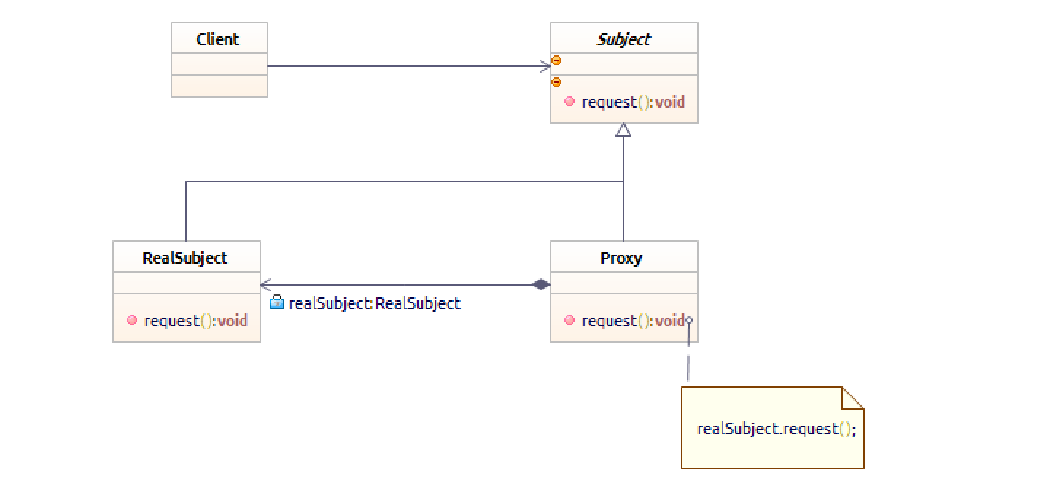
\includegraphics[width=.7\linewidth]{imagenes/Patrones/estructura_Proxy.pdf}
	\caption{Estructura del patrón Proxy.\cite{gof}}	
\end{figure}

\paragraph{Actores}

\begin{itemize}
	\item \textbf{Proxy}: Controla el acceso al sujeto real y puede ser responsable de crearlo y eliminarlo.
	\item \textbf{Sujeto}:Define la interfaz común para las clase SujetoReal y Proxy para que un Proxy se pueda usar en cualquier lugar donde se espere un SujetoReal.
	\item \textbf{Sujeto Real}:Define el objeto real al cual representa el Proxy.
\end{itemize}


\subsubsection{Caso de Uso}


